% ------------------------------------------------------------------------
% file `arbeitsblatt-example-1-exercise-body.tex'
%
%     exercise of type `example' with id `1'
%
% generated by the `example' environment of the
%   `xsim' package v0.11 (2018/02/12)
% from source `arbeitsblatt' on 2020/10/28 on line 183
% ------------------------------------------------------------------------
Eine Ampel kann als endlicher Automat betrachtet werden. Am Anfang ist sie rot, nach einer gewissen Zeit wird sie (zumindest in Deutschland) rot-gelb, dann wird sie grün, dann gelb und schliesslich wird sie wieder rot und der Zyklus geht von vorne los. Schematisch können wir das Verhalten dieser Ampel mit einem gerichteten Graphen darstellen. Wir zeichnen einen Knoten für jede Ampelfarbe und verwenden gerichtete Kanten, um zu zeigen, wie sich die Farben ändern.
\begin{figure}[H]
\centering
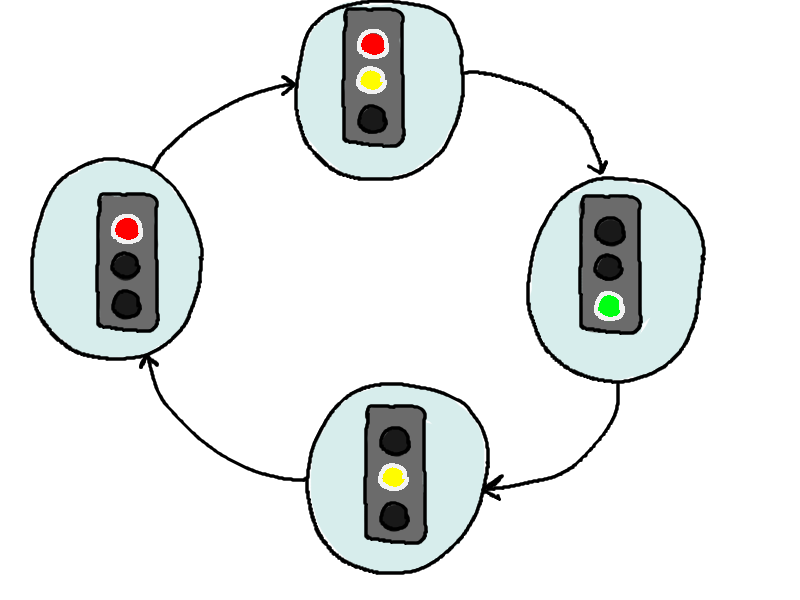
\includegraphics[width=0.4\linewidth]{Pictures/Ampel.png}
\end{figure}
